\ifx\allfiles\undefined
\documentclass[8pt a4paper, oneside, UTF8]{ctexbook}  % +  这一句是新增加的
\input{../config/config}
\begin{document}
\begin{sloppypar}
    % \title{{\Huge{\textbf{考研高等数学笔记}}}}
\author{作者:LoafPhilosopher }
\date{\today}
\maketitle                   % 在单独的标题页上生成一个标题
\thispagestyle{empty}        % 前言页面不使用页码
% \begin{center}
% 	\Huge\textbf{前言}
% \end{center}
% 本笔记主要结合张宇老师和武忠祥老师的以及邂逅遗憾老师的内容进行编写
% \begin{flushright}
% 	\begin{tabular}{c}
% 		\today \newline 
% 	\end{tabular}
% \end{flushright}
\newpage                      % 新的一页
\pagestyle{plain}             % 设置页眉和页脚的排版方式(plain:页眉是空的,页脚只包含一个居中的页码)
\setcounter{page}{1}          % 重新定义页码从第一页开始
\pagenumbering{Roman}         % 使用大写的罗马数字作为页码

\begin{spacing}{1.5}
	\tableofcontents
\end{spacing}           % 生成目录
\newpage                      % 以下是正文
\pagestyle{plain}
\setcounter{page}{1}          % 使用阿拉伯数字作为页码
\pagenumbering{arabic}
% \setcounter{chapter}{-1}    % 设置 -1 可作为第零章绪论从第零章开始 
    \else
    \fi
    %  ############################ 正文部分
    \chapter{导数}
    \section{导数的概念}
    \subsection{导数的定义}
    \begin{defn}{导数的定义}{}
        设函数$y=f(x)$在点 $x_0$的某个邻域内有定义,当自变量 $x$ 在 $x_0$处取得增量 $\Delta x$(点$x_0+\Delta x$仍在该邻域内)时,相应地,因变量取得增量$\Delta y=f(x_0+\Delta x)-f(x_0)$;如果$\Delta  y$与$\Delta x$之比当 $\Delta x \to 0$时的极限存在,那么称函数 $y=f(x)$在点 $x_0$处可导,并称这个极限为函数 $y=f(x)$在点 $x_0$处的\textbf{导数},记为$f^{\prime}(x_0)$,即
        $$
            f^{'}(x_{0})=\lim_{x\to x_{0}}\frac{f(x)-f(x_{0})}{x-x_{0}}=\lim_{\Delta x\to0}\frac{\Delta y}{\Delta x}=\lim_{\Delta x\to0}\frac{f(x_{0}+\Delta x)-f(x_{0})}{\Delta x}
        $$
        也可记作$\left.y^{\prime}\right|_{x=x_{0}},\left.\dfrac{\mathrm{d}y}{\mathrm{d}x}\right|_{x=x_{0}}\text{或}\left.\dfrac{\mathrm{d}f(x)}{\mathrm{d}x}\right|_{x=x_{0}}.$
    \end{defn}
    \begin{criterion}{导数定义的注意事项}{}
        \begin{enumerate}
        \item 在考题中,增量$\Delta x$一般会被命题人广义化为"$\square$",即
        $$
            f'(x_0)=\lim_{\Delta x \to 0}\frac{f(x_0+\Delta x)-f(x_0)}{\Delta x}\xlongequal{\text{广义化}} \lim_{ \square \to 0}\frac{f(x_0 + \square)-f(x_0)}{\square}
        $$
        需要知道的是$\square$需要同时趋近于$0^+$和$0^-$该点导数才存在,如果仅趋近于其中的一个,则是$\square$处的单侧导数\\
        若在上式中,令$x_0+\Delta x=x$,则可将导数定义式写成
        $$
            f^{\prime}(x_{0})=\lim_{x\to x_{0}}\dfrac{f\left(x\right)-f\left(x_{0}\right)}{x-x_{0}}
        $$
        \item 以下的三种说法是等价的:
            \begin{itemize}
                \item  $y=f\left(x\right)$在点$x_{0}$处可导
                \item $y=f\left(x\right)$在点$x_{0}$处导数存在
                \item  $f^{\prime}\left(x_{0}\right)=A\left(A\text{为有限数}\right)$
            \end{itemize}
        \item \textcolor{red}{导数若存在,则导数要么连续,要么只可能有震荡间断点}
        \begin{proof}[导数若存在有震荡间断点的证明:]
            以函数$F(x)=\begin{cases}
                x^2 \sin \dfrac{1}{x} ,x \neq 0\\
                0,x=0
            \end{cases}$为例:
            \\根据导数定义对函数在$x=0$处求导:$F'(0)=\lim_{x\to 0}\dfrac{F(x)-F(0)}{x-0}=\lim_{x\to 0}\dfrac{x^2 \sin \frac1x - 0}{x}=\lim_{x\to 0}x \sin \dfrac{1}{x}=0$因此函数$F(x)$在$x=0$处导数存在.那么对函数求导:\\
            $F'(x)=\begin{cases}
                2x \sin \dfrac{1}{x} -\cos \dfrac{1}{x} ,x\neq 0\\
                0 ,x=0
            \end{cases}$,那么易知$\lim_{x\to 0}\left(2 x \sin \dfrac{1}{x} -\cos \dfrac{1}{x} \right)$是震荡的.虽然函数导数存在,但是这是震荡间断点.
        \end{proof}
        同时,导数震荡的话,则导数极限不存在,由此可以推出衍生推论:导数极限定理\ref{dsjxdl}
        \item 原函数可导无法推出导函数连续
        \item \textbf{函数在一点可导的必要条件:若$f(x)$在一点可导,则$f(x)$在该点连续}
        \item \textcolor{red}{需要区分一点处的右导数和导数的右极限}
            \begin{itemize}
                \item $f_+'(x_0) \Rightarrow$表示一点处的右导数$\Rightarrow \lim_{x \to x_0^+}\dfrac{f(x)-f(x_0)}{x-x_0}$
                \item $f'(x_0 ^+)=f'(x_0+0) \Rightarrow$导数的右极限$\Rightarrow \lim_{x\to x_0^+}f'(x)$
                \item $f(x_{0}^{+})=f(x_{0}+0) \Rightarrow$函数的右极限$\Rightarrow \lim_{x\to x ^+ _0}f(x)$
            \end{itemize}
        如果函数$f(x)$连续可导或者$f'(x)$连续,那么$f_+'(x_0)=f'(x_0^+)$,即右导数等于右极限.如果不连续,以函数$f(x)=\begin{cases}
            x,x \leqslant 0\\
            x+1,x >0
        \end{cases}$为例:
        显然该函数在$x=0$处不连续.那么:
        \begin{itemize}
            \item 左导数:$f_-^{\prime}(0)=\lim_{x\to0^{-}}\dfrac{f(x)-f(0)}{x}=\lim_{x\to0^{-}}\dfrac{x-0}{x}=1$
            \item 右导数:$f_{+}^{\prime}(0)=\lim_{x\to0}\dfrac{f(x)-f(0)}{x}=\lim_{x\to0^{+}}\dfrac{x+1-0}{x}=\dfrac{1}{0}=\infty $
            \item 导数的右极限:$\lim_{x \to 0^+}f'(x)=\lim_{x\to 0^+}(x+1)' = 1$
        \end{itemize}
        \end{enumerate}
    \end{criterion}
    \begin{problem}
        若$f(x)$在点$x_{0}$处的左,右导数都存在,则 $f(x)$在点$x_{0}$处\\
        (A) 可导 \quad (B)连续 \quad  (C)不可导 \quad (D)不一定连续
    \end{problem}
    \begin{solution}
        左右导数存在说明左右可导,左可导说明左连续,右可导说明右连续.左连续说明左侧极限等于该点函数值,右连续说明右侧极限等于该点函数值,那么左右极限相等且等于该点函数值,那么函数在该点连续.因此B选项正确.
    \end{solution}
    \begin{problem}
        设$f(0)=0$,则$f(x)$在点$x=0$可导的充要条件为\\
        (A)$\lim_{h\to0}\dfrac{1}{h^{2}}f(1-\cos h)$存在\quad(B)$\lim_{h\to0}\dfrac{1}{h}f(1-e^h)$ 存在\\
        (C)$\lim_{h\to0}\dfrac1{h^2}f(h-\sin h)$ 存在\quad(D)$\lim_{h\to0}\dfrac{1}{h}[f(2h)-f(h)]$存在
    \end{problem}
    \begin{solution}
        A: $\lim_{h \to 0}\dfrac{f(1 -\cos h)-f(0)}{h^2}=\lim_{h \to 0}\dfrac{f(1-\cos h)-f(0)}{1-\cos h}\cdot \dfrac{1-\cos h}{h^2}$,若$h \to 0$可以知道的是$1- \cos h$趋近于$0^+$,$\dfrac{1 - \cos h}{h^2} \to 1$,那么$\dfrac{1}{2}f_+'(0)$存在\\
        B: $\lim_{h \to 0}\dfrac{1}{h}f(1-e^h)=\lim_{h \to 0}\dfrac{1-e^h}{h}\dfrac{f(1-e^h)-f(0)}{1-e^h}$,易知$1-e^h$同时趋近于$0^+$和$0^-$,那么函数$f'(0)$存在\\
        C:$\lim_{h \to 0}\dfrac{1}{h^2}f(h- \sin h)=\lim_{h\to 0}\dfrac{f(h-\sin h)-f(0)}{h^2}=\lim_{h \to 0}\dfrac{f(h-\sin h)}{h -\sin h}\cdot \dfrac{h-\sin h}{h^2}$,已知$h -\sin h \sim \dfrac{1}{6}h^3$,那么$\lim_{h \to 0}\dfrac{f(h-\sin h)}{h -\sin h}\cdot \dfrac{h}{1}$极限存在,同时$h \to 0$,但是不可以推出$\dfrac{f(h-\sin h)}{h-\sin h}$极限存在,只能得到该极限是为定式,那么更无法推出该导数存在\\
        D:若$\lim_{h \to 0}\dfrac{1}{h}[f(2h)-f(h)]$存在,那么其实什么都推不出来,因为不知道$\dfrac{f(2h)}{h}$和$\dfrac{f(h)}{h}$是否存在,如果写成下列形式$\lim_{h \to 0}\dfrac{[f(2h)-f(0)]-[f(h)-f(0)]}{h}=\lim_{h \to 0}\left(\dfrac{f(2h)-f(0)}{h}-\dfrac{f(h)-f(0)}{h}\right)$,则违反了极限的运算法则.\\
        综上答案选择B选项
    \end{solution}
    \begin{note}
        \textcolor{red}{若想推出$f(x)$在$x=0$处可导,则必须满足下面的四个条件:}
        \begin{enumerate}
            \item 一动减一定:必须是一个动点减一个定点.比如上题中的D选项,本质上是两个动点相减.
            \item 可正可负:指的是分母,即定义中的$\square$,需要同时趋近于$0^+$和$0^-$,如果只能趋近于一个,则为单侧导数.
            \item 上下同阶:即分子的阶数小于等于分母阶数.但是如果要求是充要条件则必须是同阶.比如下面的例子:
            若$\lim_{x\to 0}\dfrac{f(x-\sin x)-f(0)}{x^4}$存在,那么$\lim_{x\to 0}\dfrac{f(x-\sin x)-f(0)}{x-\sin x}\cdot \dfrac{x - \sin x}{x^4}$,其中$ x - \sin x \sim \dfrac{1}{6}x^3$,那么$\lim_{x\to 0}\dfrac{f(x-\sin x)-f(0)}{(x-\sin x)-0}\cdot \dfrac{1}{6x}$,其中$\lim_{x\to 0} \dfrac{1}{6x} \to \infty$,那么$\lim_{x\to 0}\dfrac{f(x-\sin x)-f(0)}{(x-\sin x)-0}$必定存在且$\dfrac{f(x-\sin x)-f(0)}{(x-\sin x)-0}=0 \Rightarrow f'(0)=0$
            \item 填满邻域:在定义中的$\square$需要把其附近邻域都给填满.比如下面的例子:$\lim_{n\to \infty}\dfrac{f(\frac{1}{n})-f(0)}{\frac{1}{n}}=0$,无法推出$f'_+(0)=0$存在,因为$\dfrac{1}{n}$取不到无理数,无法包含$\square$邻域
        \end{enumerate}
    \end{note}
    \begin{them}{导数极限定理}{}\label{dsjxdl}
        如果$f(x)$在$x_0$的邻域内连续,在$x_{0}$的去心邻域内可导,且导函数在$x_{0}$处的极限存在(等于$a$),则$f(x)$在$x_0$处的导数也存在并且等于导函数的极限(等于$a$)
    \end{them}
        上述定理可解释为导函数如果在某点极限存在,那么在该点导函数一定连续.因为导数存在要么有震荡间断点,要么连续.如果说该点导函数极限存在,那么一定连续.
    \begin{problem}
        设$f(x)$ 在 $x=x_0$ 处有二阶导数,则\\
        (A) 当$f(x)$在$x_0$的某邻域内单调增加时,$f^\prime(x_0)>0.$
        (C)当$f(x)$在$x_0$的某邻域内是凹函数时,$f^{\prime\prime}(x_0)>0.$\\
        (B)当$f^\prime(x_0)>0$时,$f(x)$在$x_0$的某邻域内单调增加
        (D)当$f^{\prime\prime}(x_0)>0$时,$f(x)$在$x_0$的某邻域内是凹函数
    \end{problem}
    \begin{solution}
        A:当$f(x)$在$x_0$某邻域内单调增加时,
    \end{solution}
    \begin{note}
            
    \end{note}
    \begin{problem}
        已知 $f(x)$ 在 $x=0$ 处连续,且$\lim_{x\to 0}\dfrac{x^2}{f(x)}=1$,则下列结论中正确的个数为\\
        (1)$f^{\prime}(0)$ 存在,且 $f^\prime(0)=0.$ \quad (2)$f^{\prime\prime}(0)$ 存在,且 $f^{\prime\prime}(0)=2.$\\
        (3)$f(x)$在$x=0$处取得极小值\quad (4)$f\left(x\right)$在 $x=0$ 的某邻域内连续.
    \end{problem}
    \begin{solution}
            
    \end{solution}
    \begin{note}
            
    \end{note}
    \begin{problem}
        设函数$f(x)$在$(-1,1)$上有定义,且$\lim_{x\to0}f(x)=0$,则\\
        (A)当$\lim_x\to0\dfrac{f(x)}{\sqrt{|x|}}=0$时$,f(x)$在$x=0$处可导
        (B)当$\lim_x\to0\dfrac{f(x)}{x^{2}}=0$时$,f(x)$在$x=0$处可导\\
        (C)当$f(x)$在$x=0$处可导时$,\lim_{x\to0}\dfrac{f(x)}{\sqrt{|x|}}=0$\quad
        (D)当$f(x)$在$x=0$处可导时$,\lim_{x\to0}\dfrac{f(x)}{x^{2}}=0$        
    \end{problem}
    \begin{solution}
            
    \end{solution}
    \begin{note}
            
    \end{note}
    \begin{problem}
        设 $f(x)$ 可导且 $f^\prime(x_0)=\dfrac12$,则当$\Delta x\to0$ 时$,f(x)$在$x_0$处的微分$\operatorname{dy}$是$\Delta x$ 的无穷小.\\
        A.等价 \quad B.同阶 \quad C.低阶 \quad D.高阶
    \end{problem}
    \begin{solution}
            
    \end{solution}
    \begin{note}
            
    \end{note}
    \begin{problem}
        已知函数$f(x)\:=\begin{cases}x,&x\leqslant0,\\\dfrac{1}{n},&\dfrac{1}{n+1}<x\leq\dfrac{1}{n},n\:=\:1,2,\cdots,\end{cases}$则:\\
        (A)$x=0$ 是$f(x)$ 的第一类间断点. \quad
        (C)$f(x)$在$x=0$处连续但不可导.\\
        (B) $x$ = 0 是$f(x)$ 的第二类间断点.\quad
        (D)$f(x)$在$x=0$处可导.
    \end{problem}
    \begin{solution}
            
    \end{solution}
    \begin{note}
            
    \end{note}
    \begin{problem}
        下列命题正确的个数为:\\
        1.设$\lim_{x\to x_0^-}f^{\prime}(x)$与$\lim_{x\to x_0^+}f^{\prime}(x)$均存在,则 $f(x)$ 在 $x=x_0$ 处必连续\\
        2.设$f^{\prime}_-(x_{0})$与$f^{\prime}_{+}(x_{0})$ 均存在,则$f(x)$在$x=x_{0}$处必连续\\
        3.设$f(x_{0}^{-})$与$f(x_{0}^{+})$均存在,则$f(x)$在$x=x_{0}$处必连续\\
        4.设$\lim_{x\to x_{0}^{-}}f^{\prime}(x)$与$\lim_{x\to x_{0}^{+}}f^{\prime}(x)$中至少有一个不存在,则 $f(x)$ 在 $x=x_0$ 处必不可导
    \end{problem}
    \begin{solution}
            
    \end{solution}
    \begin{note}
            
    \end{note}
    \subsection{单侧导数}
    \begin{defn}{单侧导数的定义}{}
            函数$f(x)$在$x_0$点可导的充分必要条件是左导数和右导数存在且相等,其表达式为
            $$
                \begin{aligned}&\lim_{h \to0^-}\frac{f(x_0+h )-f(x_0)}{h }\xlongequal{\text{记}}f'_{-}\left(x_0\right)\\&\lim_{h \to0^+}\frac{f(x_0+h )-f(x_0)}{h }\xlongequal{\text{记}}f'_{+}\left(x_0\right)\end{aligned}
            $$
    \end{defn}
    \begin{criterion}{一点可导与邻域的关系}{}
        \begin{itemize}
            \item 一点可导$\neq$点邻域可导:以函数$f(x)=x^2 D(x)=\begin{cases}
                x^2,x\in\text{有理数}\\0,x\in \text{无理数}
            \end{cases}$为例
            \item 一点可导邻域内连续:若函数在一点可导,则函数在该点连续,而无法断言函数在这点附近的连续性,仍可以$f(x)=x^2 D(x)$为例
        \end{itemize}
    \end{criterion}

    \subsection{导数的几何意义}
    \begin{defn}{导数的几何意义}{}
        $y=f(x)$在$x_0$处导数是$f(x)$在$x_0$处切线的斜率$k_\text{切} = f ^ { \prime } ( x _ { 0 } )$并且$k_\text{切}*k_\text{法}=-1$\\
        在($x_0$,$y_0$)处,切线方程:$$y-y_{0}=f^{\prime}(x_{0})(x-x_{0})$$
        \begin{center}
            \vspace{-0.8cm}
            \tikzset{every picture/.style={line width=0.85pt}} %set default line width to 0.75pt        
            \begin{tikzpicture}[x=0.75pt,y=0.75pt,yscale=-1,xscale=1]
                \draw  (197,243.01) -- (388.14,243.01)(216.11,94) -- (216.11,259.57) (381.14,238.01) -- (388.14,243.01) -- (381.14,248.01) (211.11,101) -- (216.11,94) -- (221.11,101)  ;
                \draw   (235,228) .. controls (286.38,33.14) and (337.76,325.43) .. (389.14,130.57) ;
                \draw  [dash pattern={on 4.5pt off 4.5pt}]  (306.14,140.57) -- (236.14,176.57) ;
                \draw (201,247) node [anchor=north west][inner sep=0.75pt]   [align=left] {$\displaystyle O$};
                \draw (212,70) node [anchor=north west][inner sep=0.75pt]   [align=left] {$\displaystyle y$};
                \draw (381,249) node [anchor=north west][inner sep=0.75pt]   [align=left] {$\displaystyle x$};
                \draw (241,133) node [anchor=north west][inner sep=0.75pt]  [font=\footnotesize] [align=left] {$\displaystyle ( x_{0} ,y_{0})$};
            \end{tikzpicture}
            \vspace{-2cm}
        \end{center}
        如上图所示,点$(x_0,y_0)$处的切线为虚线\\
        法线方程:$$y-y_{0}=-\dfrac{1}{f^{\prime}(x_{0})}(x-x_{0})$$
    \end{defn}
    \begin{criterion}{角点与无穷导数}{}
        \begin{itemize}
            \item 研究$y=f(x)=|x|$在$x=0$处的切线问题
            \begin{solution}
                从$x=0$出发,取增量$\Delta x$,有$\Delta y=f\left(0+\Delta x\right)-f\left(0\right)=\left|\Delta x\right|$\\
                当$\Delta x>0$时,$\Delta y=\Delta x,$则$f_{+}^{\prime}(0)=\lim_{\Delta x\to0^{+}}\dfrac{\Delta y}{\Delta x}=1\xlongequal{\text{记}}k_{+}$\\当$\Delta x<0$时,$\Delta y=-\Delta x,$则$f_{-}^{\prime}(0)=\lim_{\Delta x\to0^{-}}\dfrac{\Delta y}{\Delta x}=-1\xlongequal{\text{记}}k_{-}$
                \begin{center}
                    \tikzset{every picture/.style={line width=0.75pt}} %set default line width to 0.75pt        
                    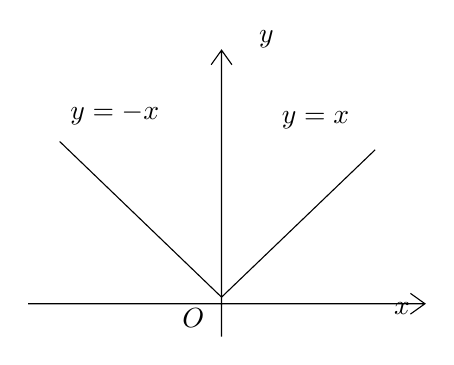
\begin{tikzpicture}[x=0.75pt,y=0.75pt,yscale=-1,xscale=1]
                    \draw  (95,215.74) -- (286.14,215.74)(188.14,93.57) -- (188.14,231.57) (279.14,210.74) -- (286.14,215.74) -- (279.14,220.74) (183.14,100.57) -- (188.14,93.57) -- (193.14,100.57)  ;
                    \draw    (110.14,137.57) -- (188.14,212.57) ;
                    \draw    (262.14,141.57) -- (188.14,212.57) ;
                    \draw (168,217) node [anchor=north west][inner sep=0.75pt]   [align=left] {$\displaystyle O$};
                    \draw (205,83) node [anchor=north west][inner sep=0.75pt]   [align=left] {$\displaystyle y$};
                    \draw (270,214) node [anchor=north west][inner sep=0.75pt]   [align=left] {$\displaystyle x$};
                    \draw (114,118) node [anchor=north west][inner sep=0.75pt]   [align=left] {$\displaystyle y=-x$};
                    \draw (216,122) node [anchor=north west][inner sep=0.75pt]   [align=left] {$\displaystyle y=x$};
                    \end{tikzpicture}
                \end{center}
            \end{solution}
            \item 研究$y=f\left(x\right)=x^{\frac13}$在$x=0$处的切线问题
            \begin{solution}
                显然,在$x=0$ 处$\dfrac{\Delta y}{\Delta x}=\dfrac{f(0+\Delta x)-f(0)}{\Delta x}=\dfrac{(\Delta x)^{\frac13}}{\Delta x}=\dfrac{1}{(\Delta x)^{\frac{2}{3}}}$
                当$\Delta x>0$ 时,$f_{+}^{\prime}(0)=\lim_{\Delta x\to0^{+}}\dfrac{1}{\left(\Delta x\right)^{\frac{2}{3}}}=+\infty$
                 $\Delta x<0$ 时,$f_{-}^{\prime}(0)=\lim_{\Delta x\to0^{-}}\dfrac{1}{\left(\Delta x\right)^{\frac{2}{3}}}=+\infty$ 
                这样的结果称为无穷导数.又$±\infty$被叫作广义的数,所以无穷导数在有些数学场合也可被视为导数存在的特殊情形.但是在考研中无穷被认为是不存在                
            \end{solution}
        \end{itemize}
    \end{criterion}
    \subsection{高阶导数}
    \begin{defn}{高阶导数的定义}{}
        函数$y=f(x)$具有$n$阶导数,也常说成函数$f(x)$为$n$阶可导,如果函数$f(x)$在点$x$处具有$n$阶导数,那么$f(x)$在点$x$的某一邻域内必定具有一切低于$n$阶的导数.二阶及二阶以上的导数统称为高阶导数.
        记作:
        $$
        f^{(n)}(x_0)=\lim_{\Delta x\to0}\dfrac{f^{(n-1)}(x_0+\Delta x)-f^{(n-1)}(x_0)}{\Delta x}\text{或}f^{(n)}(x_0)=\lim_{x\to x_0}\dfrac{f^{(n-1)}(x)-f^{(n-1)}(x_0)}{x-x_0}
        $$
        当$n=2$时:
        $$
        f^{\prime\prime}(x_0)=\lim_{\Delta x\to0}\dfrac{f^{\prime}(x_0+\Delta x)-f^{\prime}(x_0)}{\Delta x}\text{或}f^{\prime\prime}(x_0)=\lim_{x\to x_0}\dfrac{f^{\prime}(x)-f^{\prime}(x_0)}{x-x_0}
        $$
    \end{defn}
    \section{微分}
    \subsection{微分的概念}
    \begin{defn}{微分的定义}{}
        设函数$y=f(x)$在某区间内有定义,$x_0$及$x_0+\Delta x$在这个区间内,如果函数的增量为
        $$
            \Delta y=f(x_{0}+\Delta x)-f(x_{0})
        $$
        可表示为
        $$
            \Delta y=A\Delta x+o(\Delta x)
        $$
        其中$A$是不依赖于$\Delta x$的常数,那么称函数$f(x)$在点$x_0$是可微的,而$A\Delta x$叫做函数$y=f(x)$在点$x_0$相应于自变量增量$\Delta x$​的微分,记作$dy$,即:
        $$
            dy=A\Delta x
        $$
        函数$f(x)$在任意点$x_0$的微分,称为函数的微分,记作$dy$或$df(x_0)$,即
        $$
            \textcolor{red}{dy=f^{\prime}(x)\Delta x}
        $$
    \end{defn}
    \subsection{微分的几何意义}
    若$f(x)$在点$x_{0}$处可微,则在点$(x_0,y_0)$附近可以用切线段近似代替曲线段,这是可微的几何意义.
    \begin{center}
        \tikzset{every picture/.style={line width=0.75pt}} %set default line width to 0.75pt        
        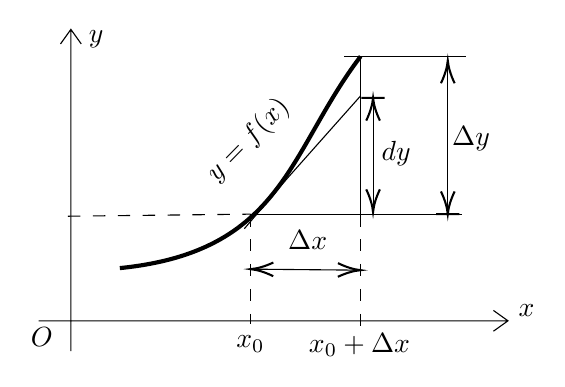
\begin{tikzpicture}[x=0.75pt,y=0.75pt,yscale=-1,xscale=1]
        \draw  (95,216.97) -- (321.14,216.97)(110.55,76.57) -- (110.55,231.57) (314.14,211.97) -- (321.14,216.97) -- (314.14,221.97) (105.55,83.57) -- (110.55,76.57) -- (115.55,83.57)  ;
        \draw [line width=1.5]    (250.14,89.57) .. controls (215.14,135.57) and (213.14,183.57) .. (134.14,191.57) ;
        \draw    (194.14,172.57) -- (214.88,148.26) -- (250.14,108.57) ;
        \draw  [dash pattern={on 4.5pt off 4.5pt}]  (109.14,166.57) -- (197.14,165.57) ;
        \draw  [dash pattern={on 4.5pt off 4.5pt}]  (197.14,165.57) -- (197.14,218.57) ;
        \draw    (197.14,165.57) -- (299.14,165.57) ;
        \draw    (250.14,108.57) -- (250.14,165.57) ;
        \draw  [dash pattern={on 4.5pt off 4.5pt}]  (250.14,165.57) -- (250.14,219.57) ;
        \draw    (242.14,89.57) -- (301.14,89.57) ;
        \draw    (292.14,93.57) -- (292.14,165.57) ;
        \draw [shift={(292.14,165.57)}, rotate = 270] [color={rgb, 255:red, 0; green, 0; blue, 0 }  ][line width=0.75]    (0,5.59) -- (0,-5.59)(10.93,-3.29) .. controls (6.95,-1.4) and (3.31,-0.3) .. (0,0) .. controls (3.31,0.3) and (6.95,1.4) .. (10.93,3.29)   ;
        \draw [shift={(292.14,91.57)}, rotate = 90] [color={rgb, 255:red, 0; green, 0; blue, 0 }  ][line width=0.75]    (10.93,-3.29) .. controls (6.95,-1.4) and (3.31,-0.3) .. (0,0) .. controls (3.31,0.3) and (6.95,1.4) .. (10.93,3.29)   ;
        \draw    (256.14,109.57) -- (256.14,162.57) ;
        \draw [shift={(256.14,164.57)}, rotate = 270] [color={rgb, 255:red, 0; green, 0; blue, 0 }  ][line width=0.75]    (10.93,-3.29) .. controls (6.95,-1.4) and (3.31,-0.3) .. (0,0) .. controls (3.31,0.3) and (6.95,1.4) .. (10.93,3.29)   ;
        \draw [shift={(256.14,109.57)}, rotate = 90] [color={rgb, 255:red, 0; green, 0; blue, 0 }  ][line width=0.75]    (0,5.59) -- (0,-5.59)(10.93,-3.29) .. controls (6.95,-1.4) and (3.31,-0.3) .. (0,0) .. controls (3.31,0.3) and (6.95,1.4) .. (10.93,3.29)   ;
        \draw    (250.14,89.57) -- (250.14,108.57) ;
        \draw    (248.14,192.55) -- (199.14,192.09) ;
        \draw [shift={(197.14,192.07)}, rotate = 0.54] [color={rgb, 255:red, 0; green, 0; blue, 0 }  ][line width=0.75]    (10.93,-3.29) .. controls (6.95,-1.4) and (3.31,-0.3) .. (0,0) .. controls (3.31,0.3) and (6.95,1.4) .. (10.93,3.29)   ;
        \draw [shift={(250.14,192.57)}, rotate = 180.54] [color={rgb, 255:red, 0; green, 0; blue, 0 }  ][line width=0.75]    (10.93,-3.29) .. controls (6.95,-1.4) and (3.31,-0.3) .. (0,0) .. controls (3.31,0.3) and (6.95,1.4) .. (10.93,3.29)   ;
        \draw (90,219) node [anchor=north west][inner sep=0.75pt]   [align=left] {$\displaystyle O$};
        \draw (118,76) node [anchor=north west][inner sep=0.75pt]   [align=left] {$\displaystyle y$};
        \draw (325,208) node [anchor=north west][inner sep=0.75pt]   [align=left] {$\displaystyle x$};
        \draw (171.74,143.51) node [anchor=north west][inner sep=0.75pt]  [rotate=-314.36] [align=left] {$\displaystyle y=f( x)$};
        \draw (293,122) node [anchor=north west][inner sep=0.75pt]   [align=left] {$\displaystyle \Delta y$};
        \draw (259,129) node [anchor=north west][inner sep=0.75pt]   [align=left] {$\displaystyle dy$};
        \draw (189,223) node [anchor=north west][inner sep=0.75pt]   [align=left] {$\displaystyle x_{0}$};
        \draw (224,222) node [anchor=north west][inner sep=0.75pt]   [align=left] {$\displaystyle x_{0} +\Delta x$};
        \draw (214,172) node [anchor=north west][inner sep=0.75pt]   [align=left] {$\displaystyle \Delta x$};
        \end{tikzpicture}
    \end{center}
    \section{导数的计算}
    \subsection{基本求导公式}
    \begin{center}
        \boxed{
            $$
                \begin{aligned}
                     & \left(C\right)^{\prime}=0;                        &  & \left(x^{\alpha}\right)^{\prime}=\alpha x^{\alpha-1}; \\
                     & \left(a^{x}\right)^{\prime}=a^{x}\ln a;           &  & \left(\mathrm{e}^{x}\right)^{\prime}=\mathrm{e}^{x};  \\
                     & \left(\log_{a}x\right)^{\prime}=\dfrac{1}{x\ln a}; &  & (\ln|x|)^{\prime}=\dfrac{1}{x};                                   \\
                     & \left(\sin x\right)^{\prime}=\cos x;              &  & \left(\cos x\right)^{\prime}=-\sin x;                 \\
                     & \left(\tan x\right)^{\prime}=\sec^{2}x;           &  & \left(\cot x\right)^{\prime}=-\csc^{2}x;             \\
                     & (\sec x)'=\sec x\tan x;                                     &  & (\csc x)'=-\csc x\cot x;                                        \\
                     & (\arcsin x)'=\dfrac{1}{\sqrt{1-x^2}};                        &  & (\arccos x)'=-\frac{1}{\sqrt{1-x^2}};                           \\
                     & (\arctan x)'=\dfrac{1}{1+x^2};                               &  & (\operatorname{arccot}x)'=-\frac{1}{1+x^2}.\\
                     & [\ln(x+\sqrt{x^2+1})]^{\prime}=\dfrac{1}{\sqrt{x^2+1}};                               &  & [\ln(x+\sqrt{x^{2}-1})]^{\prime}=\dfrac{1}{\sqrt{x^{2}-1}} 
                    \end{aligned}
            $$
        }
    \end{center}
    \subsection{有理运算法则}
    设$u=u(x),v=v(x)$在$x$处可导,则
    $$
        (u\pm v)^{\prime}=u^{\prime}\pm v^{\prime}
    $$
    $$
        \left(uv\right)^{\prime}=u^{\prime}v+uv^{\prime}
    $$
    $$
        \left(\frac uv\right)^{\prime}=\dfrac{u^{\prime}v-uv^{\prime}}{v^2}\quad(v\neq0)
    $$
    \subsection{复合函数的导数与微分形式不变性}
    \subsubsection{复合函数导数}
    \begin{defn}{复合函数导数的定义}{}
        设$y = f ( g ( x ) )$是由$y=f(z)$,$z=g(x)$复合而成,且$f(z)$,$g(x)$均可导,则$\{f[g(x)]\}'=f'[g(x)]g'(x)$
    \end{defn}
    \subsubsection{微分形式不变形}
    \begin{defn}{微分形式不变形}{}
        设$u=g(x)$在点$x$(没有下标是泛指的点,下同)处可导,$y=f(u)$在点$u=g(x)$处可导,则
        $$
        \mathrm{d}\{f[g(x)]\}=f'[g(x)]g'(x)\mathrm{d}x=f'[g(x)]\mathrm{d}[g(x)]
        $$
        指无论$u$是中间变量还是自变量,$dy=f'(u)du$都成立.
    \end{defn}
    \subsection{分段函数的导数}
    设$f(x)=\begin{cases}f_1(x),&x\geqslant x_0,\\f_2(x),&x<x_{0},\end{cases}$其中$f_1(x),f_2(x)$分别在$x>x_0,x<x_0$时可导,则
    \begin{itemize}
        \item 在分段点$x_{\mathrm{o}}$处用导数定义求导$:f_+^{\prime}(x_0)=\lim_{x\to x_0^+}\dfrac{f_1(x)-f(x_0)}{x-x_0},f_-^{\prime}(x_0)=\lim_{x\to x_0^-}\dfrac{f_2(x)-f(x_0)}{x-x_0}$ .根据$f_+^{\prime}(x_0)$ 是否等于$f_-^{\prime}(x_0)$来判定$f^{\prime}(x_0);$
        \item 在非分段点用导数公式求导,即$x>x_0$时,$f^{\prime}(x)=f_1^{\prime}(x);x<x_0$时,$f^{\prime}(x)=f_2^{\prime}(x)$
    \end{itemize}
    \subsection{反函数的导数}
    \begin{defn}{反函数导数的定义}{}
        设$y=f(x)$为单调、可导函数,且$f^{\prime}(x)\neq0$,则存在反函数$x=\varphi(y)$,且$\dfrac{\mathrm{d}x}{\mathrm{d}y}=\dfrac{1}{\dfrac{dy}{dx}}$,即 $\varphi^{\prime}(y)=\dfrac1{f^{\prime}(x)}$
    \end{defn}
    \begin{criterion}{反函数的二阶导数}{}
        在$y=f(x)$单调,且二阶可导的情况下,若$f^{\prime}(x)\neq0$,则存在反函数$x=\varphi(y)$,记$f^{\prime}(x)=y_x^{\prime},\varphi^{\prime}\left(y\right)=x_{y}^{\prime}$,则有
        $$
            y_{x}^{\prime}=\dfrac{\mathrm{d}y}{\mathrm{d}x}=\dfrac{1}{\dfrac{\mathrm{d}x}{\mathrm{d}y}}=\frac{1}{x_{y}^{\prime}}
        $$
        $$
            y_{xx}^{\prime\prime}=\dfrac{\mathrm{d}^{2}y}{\mathrm{d}x^{2}}=\dfrac{\mathrm{d}\left(\dfrac{\mathrm{d}y}{\mathrm{d}x}\right)}{\mathrm{d}x}=\dfrac{\mathrm{d}\left(\dfrac{1}{x_{y}^{\prime}}\right)}{\mathrm{d}x}=\dfrac{\mathrm{d}\left(\dfrac{1}{x_{y}^{\prime}}\right)}{\mathrm{d}y}\cdot\dfrac{1}{x_{y}^{\prime}}=-\dfrac{1}{(x_{y}^{\prime})^{2}}\cdot(x_{y}^{\prime})_{y}^{\prime}\cdot\dfrac{1}{x_{y}^{\prime}}=-\dfrac{x_{yy}^{\prime\prime}}{(x_{y}^{\prime})^{2}}\cdot\dfrac{1}{x_{y}^{\prime}}=-\dfrac{x_{yy}^{\prime\prime}}{(x_{y}^{\prime})^{3}}
        $$
        反过来则有:
        $$
            x_{y}^{\prime}=\dfrac{1}{y_{x}^{\prime}},x_{yy}^{\prime\prime}=-\dfrac{y_{xx}^{\prime\prime}}{(y_{x}^{\prime})^{3}}
        $$
    \end{criterion}
    \subsection{参数方程求导}
    \begin{defn}{参数方程所确定的函数的导数}{}
        设$y=f(x)$的参数方程是$\left\{\begin{aligned}x&=\varphi(t),\\y&=\psi (t),\end{aligned}\right.(\alpha<t<\beta)$确定的函数

        如果$\varphi(t)$和$\psi(t)$都可导,且$\varphi'(t) \neq 0$则其一阶导可写为
        $$
            \dfrac{\mathrm{d}y}{\mathrm{d}x}=\frac{\psi^{\prime}(t)}{\varphi^{\prime}(t)}
        $$
        若$\varphi(t)$ 和$\psi(t)$ 二阶可导,且 $\varphi^{\prime}(t)\neq 0$,则
        $$
            \begin{aligned}
                \frac{\operatorname{d}^2y}{\operatorname{d}x^2} & =\frac{d}{dx}(\frac{dy}{dx}) =\frac{\operatorname{d}}{\operatorname{d}t}\Big(\frac{\psi'(t)}{\varphi'(t)}\Big) \times \frac{1}{\varphi'(t)} \\
                & =\frac{\psi''(t)\varphi'(t)-\varphi''(t)\psi'(t)}{\varphi'^2(t)}\times \frac{1}{\varphi'(t)}                                                \\
                & =\frac{\psi''(t)\varphi'(t)-\varphi''(t)\psi'(t)}{\varphi'^3(t)}
            \end{aligned}
        $$
    \end{defn}
    \subsection{对数函数求导法}
    对于多项相乘、相除、开方、乘方的式子,一般先取对数再求导 .设$y=f(x)(f(x)>0)$,则
    \begin{itemize}
        \item 等式两边取对数,得 $\ln y=\ln f(x)$
        \item 两边对自变量$x$求导(同样注意$y=f(x)$,即将$y$看作中间变量),得
        $$
            \frac{1}{y}y'=\begin{bmatrix}\ln f(x)\end{bmatrix}'\Rightarrow y'=\frac{yf'(x)}{f(x)}\
        $$
    \end{itemize}
    \subsection{幂指函数求导法}
    对于$u(x)^{v(x)}$函数,可采用$e^{v(x)\ln u(x)}$进行转换求导
    然后求导,得
    $$
        \left[u(x)^{\nu(x)}\right]^{\prime}=\left[\mathrm{e}^{\nu(x)\ln u(x)}\right]^{\prime}=u(x)^{\nu(x)}\left[\nu^{\prime}(x)\ln u(x)+\nu(x)\cdot\frac{u^{\prime}(x)}{u(x)}\right]
    $$
    \subsection{隐函数求导}
    \subsubsection{隐函数的定义}
    \begin{defn}{隐函数与显函数的定义}{}
    \begin{itemize}
        \item 隐函数:$y$与$x$的关系隐含在一个等式中,$F(x,y)=0$,如$x^2+y^2=4$
        \item  显函数:因变量与自变量在等式两端,$y$和$x$各占一边,如$y=3x$​
    \end{itemize}
    \end{defn}
    \subsubsection{隐函数求导}
    \begin{defn}{隐函数求导法则}{}
        设函数$y=y(x)$是由方程$F(x,y)=0$ 确定的可导函数则
        \begin{itemize}
            \item 方程$F(x,y)=0$ 两边对自变量$x$求导,注意$y=y(x)$,即将$y$看作中间变量,得到一个关于$y^{\prime}$ 的方程
            \item 解该方程便可求出$y^{\prime}$
        \end{itemize}
    \end{defn}
    \subsection{高阶导数求导}
    \section{导数的几何应用}
    \subsection{极值}
    \subsection{单调性判别}
    \subsection{凹凸性}
    \subsection{拐点}
    \subsection{渐近线}
    \subsection{最值}
    \subsection{函数图像绘制}
    \subsection{曲率与曲率半径}
    %  ############################ 正文部分
        \ifx\allfiles\undefined
    \end{sloppypar}
\end{document}
\fi
